\documentclass[letterpaper,10pt]{memoir}

% === AUTOR === (((
\author{\textit{Por Erick I. Rodríguez Juárez.}}
% )))

% === PAQUETES === (((
% \usepackage{makeidx}
% \usepackage{xltxtra}
\usepackage{amsfonts}
\usepackage{amsmath}
\usepackage{amssymb}
% \usepackage{fullpage}
\usepackage{tikz}
\usetikzlibrary{arrows.meta}
\usepackage{graphicx}
% )))

% === TIPOGRAFÍA === (((
% \setmainfont[
  % BoldFont       = bodonibi,
	% ItalicFont     = Century modern italic2.ttf,
	% BoldItalicFont = bodonibi,
	% SmallCapsFont  = lmromancaps10-regular.otf
% ]{Century_modern.ttf}
% )))

% === COMANDOS === (((
% \newcommand{\dis}{\displaystyle}
% \newcommand{\qed}{\hspace{0.5cm}\rule{0.16cm}{0.4cm}}
% \newcommand{\operator}[1]{\mathop{\vphantom{\sum}\mathchoice
% {\vcenter{\hbox{\huge $#1$}}}
% {\vcenter{\hbox{\Large $#1$}}}{#1}{#1}}\displaylimits}
% \newcommand{\suma}{\operator{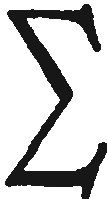
\includegraphics[scale=0.09]{FOTOS/Sigma.png}}}
% \setlength{\parindent}{0mm}
% )))

% === ITALICA EN ENTORNO MATEMÁTICO === (((
% \DeclareSymbolFont{italics}{\encodingdefault}{\rmdefault}{m}{it}
% \DeclareSymbolFontAlphabet{\mathit}{italics}
% \ExplSyntaxOn
% \int_step_inline:nnnn { `A } { 1 } { `Z }
 % {  \exp_args:Nf \DeclareMathSymbol{\char_generate:nn{#1}{11}}{\mathalpha}{italics}{#1} }
% \int_step_inline:nnnn { `a } { 1 } { `z } {  \exp_args:Nf \DeclareMathSymbol{\char_generate:nn{#1}{11}}{\mathalpha}{italics}{#1}}
% \ExplSyntaxOff
% )))

\begin{document}

\titulo

\section*{Sistemas Masa-Resorte: Movimiento Libre No-Amortiguado (3 ejercicios)} % (((
\begin{enumerate}
	\item Se fija un contrapeso de 4 lb. a un resorte cuya constante es 16 lb. /pie. ¿Cuál es el periodo del movimiento armónico simple? Esboza la gráfica del movimiento armónico simple para alguna condición específica.
		\begin{flushright}
			\textbf{Solución.} \(\dfrac{\sqrt{2} \pi}{8}\).
		\end{flushright}
	\item Al fijar un contrapeso de 24 lb. al extremo de un resorte, lo estira 4 pulg. Deduzca la ecuación del movimiento cuando el contrapeso se suelta y parte del reposo desde un punto que está 3 pulg. arriba de la posición de equilibrio. Esboza la grafica de la ecuación de movimiento.
		\begin{flushright}
			\textbf{Solución.} \(x(t) =- \dfrac{1}{4} \cos 4 \sqrt{6} t\).
		\end{flushright}
	\item Formule la ecuación del movimiento si el contrapeso del problema 2 parte de la posición de equilibrio con una velocidad inicial de 2 pie/s hacia abajo.
	\item Un contrapeso de 20 lb. estira 6 pulg. a un resorte. En ese sistema, el contrapeso se suelta, partiendo del reposo, a 6 pulgadas abajo de la posición de equilibrio.
		\begin{enumerate}
			\item Calcule la posición del contrapeso cuando \(t= \dfrac{\pi}{12} \;,\; \dfrac{\pi}{8} \;,\; \dfrac{\pi}{6} \;,\; \dfrac{\pi}{4}\), y \(\dfrac{9 \pi}{32}\) segundos.
			\item ¿Cuál es la velocidad del contrapeso cuando \(t= \dfrac{3 \pi}{16}s\)? ¿Hacia dónde se dirige el contrapeso en ese instante?
			\item ¿Cuándo pasa el contrapeso por la posición de equilibrio?
				\begin{flushright}
					\textbf{Solución.} a) \hspace{5mm}\(x \Bigg(\dfrac{\pi}{12}\Bigg) =-\dfrac{1}{4}\), \(x \Bigg(\dfrac{\pi}{8} =- \dfrac{1}{2}\Bigg)\), \(x \Bigg(\dfrac{\pi}{6}\Bigg) = -\dfrac{1}{4}\), \(x \Bigg(\dfrac{\pi}{4}\Bigg) = \dfrac{1}{2}\), \(x \Bigg(\dfrac{9 \pi}{32}\Bigg) = \dfrac{\sqrt{2}}{4}\).\\
					b) \hspace{5mm}\(4\) pies/s; hacia abajo.
					c) \hspace{5mm}\(t= \dfrac{(2n+1) \pi}{16}\), con \(n=0,1,2, \;\cdots\;\)
				\end{flushright}
		\end{enumerate}
	\item Una fuerza de 400 N estira 2 m un resorte. Después, al extremo de ese resorte se fija una masa e 50Kg. Y parte de la Posición de equilibrio a una velocidad de 10m/s hacia arriba. Deduzca la ecuación de movimiento.
	\item Otro resorte, cuya constante es 20 N/m, está colgado del mismo soporte rígido, pero en posición paralela a la del sistema masa-resorte del problema 5. Al segundo resorte se le fija una masa de 20 Kg., y ambas masas salen de su posición de equilibrio con una velocidad de 10m/s hacia arriba. hacia arriba.
		\begin{enumerate}
			\item ¿Cuál masa tiene la mayor amplitud de movimiento?
			\item ¿Cuál masa se mueve con más rapidez cuando \(t= \dfrac{\pi}{4} s\)? ¿Y cuando \(t= \dfrac{\pi}{2} s\)?
			\item ¿En qué momento están las dos masas en la misma posición? ¿Dónde están en ese momento? ¿En qué direcciones se mueven?
		\end{enumerate}
		\begin{flushright}
			\textbf{Solución.} a) La masa de \(20kg\) b) La masa de \(20kg\); la masa de \(50kg\) c) \(t=n \pi\), \(n=0,1,2, \;\cdots\;\)
		\end{flushright}
	\item Un contrapeso de 8 lb., fijo a un resorte, tiene movimiento armónico simple. Deduzca la ecuación del movimiento si la constante del resorte es 1 lb. /pie y el contrapeso parte de 6 pulg. abajo del punto de equilibrio, con una velocidad de \(\dfrac{3}{2}\) pie/s hacia abajo. Exprese la solución en la forma de la ecuación (6).
		\begin{flushright}
			\textbf{Solución.} \(x(t) = \dfrac{1}{2} \cos 2t+ \dfrac{3}{4} \sin 2t= \dfrac{\sqrt{13}}{4} \sin (2t-0.5880)\).
		\end{flushright}
\end{enumerate}
% )))

\section*{Sistemas Masa-Resorte: Movimiento Libre Amortiguado (3 ejercicios)} % (((
\begin{enumerate}
	\item La figura respectiva representa la gráfica de una ecuación del movimiento de una masa unida a un resorte. El sistema masa-resorte es amortiguado. Con la grafica, determine
		\begin{enumerate}
			\item Si el desplazamiento inicial de la masa ocurre arriba o debajo de la posición de equilibrio.
			\item Si la masa está inicialmente en reposo o si está moviéndose hacia abajo o si está moviéndose hacia arriba.
		\end{enumerate}
		\begin{center}
			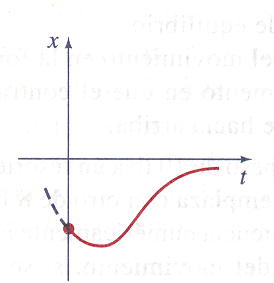
\includegraphics[height=7cm]{IMAGENES/images/image4.png}
			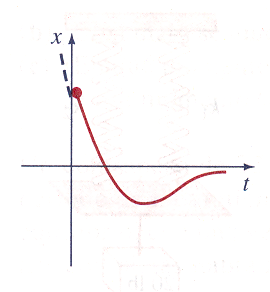
\includegraphics[height=7cm]{IMAGENES/images/image1.png}
			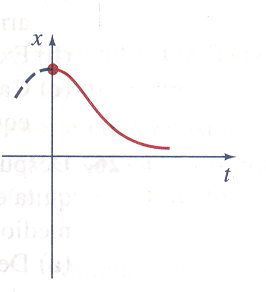
\includegraphics[height=7cm]{IMAGENES/images/image2.png}
			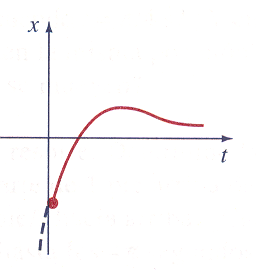
\includegraphics[height=7cm]{IMAGENES/images/image3.png}
		\end{center} 
	\item Un contrapeso de 4 lb. se une a un resorte cuya constante es 2 lb. /pie. El medio presenta una resistencia al movimiento numéricamente igual a la velocidad instantánea. Si el contrapeso se suelta de un punto a 1 pie arriba de la posición de equilibrio con una velocidad de 8 pie/s hacia abajo, calcule el tiempo en que pasa por la posición de equilibrio. Encuentre el momento en que el contrapeso llega a su desplazamiento extremo respecto a la posición de equilibrio. ¿Cuál es su posición en ese instante?
		\begin{flushright}
			\textbf{Solución.} \(\dfrac{1}{4} s\), \(\dfrac{1}{2} s\), \(x \Bigg(\dfrac{1}{2}\Bigg) =e^{-2}\); esto es, el contrapeso está, aproximadamente a \(0.14\) pies abajo de la posición de equilibrio.
		\end{flushright}
	\item Una masa de 1 Kg. está unida a un resorte cuya constante es 16 N/m y todo el sistema se sumerge en un líquido que imparte una fuerza de amortiguamiento numéricamente igual a 10 veces la velocidad instantánea. Formule las ecuaciones del movimiento, si
		\begin{enumerate}
			\item El contrapeso se suelta, partiendo del reposo a \(1 m\) abajo de la posición de equilibrio
			\item El contrapeso se suelta \(1 m\) abajo de la posición de equilibrio con una velocidad de \(12m/s\) hacia arriba.
		\end{enumerate}
		\begin{flushright}
			\textbf{Solución.} a) \(x(t) = \dfrac{4}{3} e^{-2t} - \dfrac{1}{3} e^{-8t}\). b) \(x(t) = - \dfrac{2}{3} e^{-2t} - \dfrac{5}{3} e^{-8t}\).
		\end{flushright}
	\item Una fuerza de 2 lb. estira 1 pie un resorte. A ese resorte se le une un contrapeso de 3.2 lb. Y el sistema se sumerge en un medio que imparte una fuerza de amortiguamiento numéricamente igual a 0.4 la velocidad instantánea.
		\begin{enumerate}
			\item Deduzca la ecuación del movimiento si el contrapeso parte del reposo 1 pie arriba de la posición de equilibrio.
			\item Exprese la ecuación del movimiento en la forma de la ecuación (23).
			\item Calcule el primer momento en que el contrapeso pasa por la posición de equilibrio
		\end{enumerate}
		\begin{flushright}
			\textbf{Solución.} a) \(x(t) =e^{-2t} \Bigg(- \cos 4t- \dfrac{1}{2} \sin 4t\Bigg)\). b) \(x(t) = \dfrac{\sqrt{5}}{2} e^{-2t} \sin (4t+5.176)\). c) \(t=1.294s\).
		\end{flushright}
\end{enumerate}
% )))

\section*{Sistema de Masa-Resorte: Movimiento Forzado (2 ejercicios).} % (((
\begin{enumerate}
	\item Una masa de 10 kg. esta unida a un resorte con rigidez \(k=49N/m\). Se aplica una fuerza externa \(F(t) = 20 \cos 4t\) al sistema. La constante de amortiguamiento para el sistema es de \(3N \cdot s/m\). Determina la ecuación de movimiento para el sistema y esboza su grafica.
	\item Un peso de 64 lb. esta unido a un resorte vertical, haciendo que éste se estire 3 pulgadas hasta llegar al reposo en equilibrio. La constante de amortiguamiento para el sistema es \(3lb \cdot s/pie\). Se aplica una fuerza externa \(F(t) =3 \cos 12t\). Determinar la ecuación de movimiento y esboza su grafica (si es necesario utiliza un software matemático para graficar).
\end{enumerate}
% )))

\textbf{Nota:} Revisa la resolución de las ecuaciones diferenciales usando WolfraAlpha (\url{https://www.wolframalpha.com/}) y utiliza GeoGebra (\url{https://www.geogebra.org/m/KGWhcAqc}) para graficar la ecuación de movimiento. \\[5mm]
\textbf{Bibliografía del curso:} Murray R. Spiegel, Ecuaciones Diferenciales Aplicadas, Pentice-Hall, 3er. Ed.

\end{document}
